%! Author = Omar Iskandarani
%! Title = Time Dilation in a 3D Superfluid Æther Model, Based on Vortex Core Rotation and Ætheric Flow
%! Date = May 23, 2025
%! Affiliation = Independent Researcher, Groningen, The Netherlands
%! License = CC BY-NC 4.0
%! ORCID = 0009-0006-1686-3961
%! DOI = 10.5281/zenodo.15669795

\documentclass[a4paper,12pt]{article}
\usepackage{vamstyle}
\usepackage[most]{tcolorbox}

\title{Time Dilation in a 3D Superfluid Æther Model\\  Based on Vortex Core Rotation and Ætheric Flow }
\author{
    Omar Iskandarani\thanks{
        Independent Researcher, Groningen, The Netherlands.\\
        Email: \texttt{info@omariskandarani.com}\\
        ORCID: \href{https://orcid.org/0009-0006-1686-3961}{0009-0006-1686-3961}\\
        DOI: \href{https://doi.org/10.5281/zenodo.15669902}{10.5281/zenodo.15669795}
    }
}
\date{\today}


\begin{document}
    \maketitle

    \begin{abstract}

        In this paper we derive time dilation equations within a 3D Euclidean superfluid-like æther model. In the Vortex-Æther Model (VAM) we consider a \textit{vortex} as a topologically conserved rotation field in a superfluid-like medium. In this framework, fundamental particles are modeled as vortex nodes and time is defined by the intrinsic angular rotation of their vortex cores. The goal is to replace the spacetime curvature concept of general relativity (GR) with quantized angular velocity fields in a flat-space æther, while reproducing all experimental predictions of time dilation under GR and special relativity (SR). We provide first-principles derivations, grounded in fluid dynamics and vortex mechanics, and express the time dilation factors in terms of fundamental constants such as the Planck time and maximum force. This model incorporates a multi-layered temporal formalism, distinguishing universal ætheric time $\mathcal{N}$, proper relativistic time $\tau$, and internal vortex-phase clocks $S(t)$ and $T_v$. The different modes of motion of a vortex are shown schematically in Figure~\ref{fig:rotation-translation}.

    \end{abstract}

    \begin{figure}[H]
        \centering
        \begin{tikzpicture}[scale=1.1, >=Stealth, every node/.style={font=\small}]
            % First: Pure Rotation
            \node at (-3,2.5) {Rotation};
            \draw[thick] (-3,1) circle (1);
            \draw[->, red, thick] (-4,1) -- (-4,2.2) node[left] {$R\omega = v_t$};
            \draw[->, red, thick] (-3,2) -- (-1.8,2) node[right] {$v_t$};
            \draw[->, red, thick] (-3,0) -- (-4.2,0) node[left] {$v_t$};
            \draw[->, red, thick] (-2,1) -- (-2,-0.2) node[below] {$v_t$};

            % Second: Pure Translation
            \node at (1,2.5) {Translation};
            \draw[thick] (1,1) circle (1);
            \draw[->, blue, thick] (0,1) -- (1.2,1);
            \draw[->, blue, thick] (2,1) -- (3.2,1) node[right] {$v_{cm}$};
            \draw[->, blue, thick] (1,0) -- (2.2,0);
            \draw[->, blue, thick] (1,2) -- (2.2,2);

            % Third: Combined Motion
            \node at (5.5,2.5) {Combination};
            \draw[thick] (5.5,1) circle (1);
            \draw[->, thick, purple] (5.5,2) -- (7.2,2) node[right] {$2v_{cm}$};
            \draw[->, thick, purple] (5.5,1) -- (6.7,1) node[right] {$v_{cm}$};
            \filldraw[purple] (5.5,0) circle (2pt);
            \node at (5.3,-0.3) {$0$};
        \end{tikzpicture}
        \caption{Schematic representation of three modes of motion of a vortex in the æther model. \textbf{(Left)} Pure rotation with local tangential velocity $v_t = R\omega$. \textbf{(Middle)} Translation with velocity $v_\text{cm}$ without internal rotation. \textbf{(Right)} Combining both leads to a relative velocity that differs over the vortex circumference: $v_\text{rel} = v_t + v_\text{cm}$.}
        \label{fig:rotation-translation}
    \end{figure}
    \vfill

    \newpage

    \begin{figure}[htbp]
    \centering
    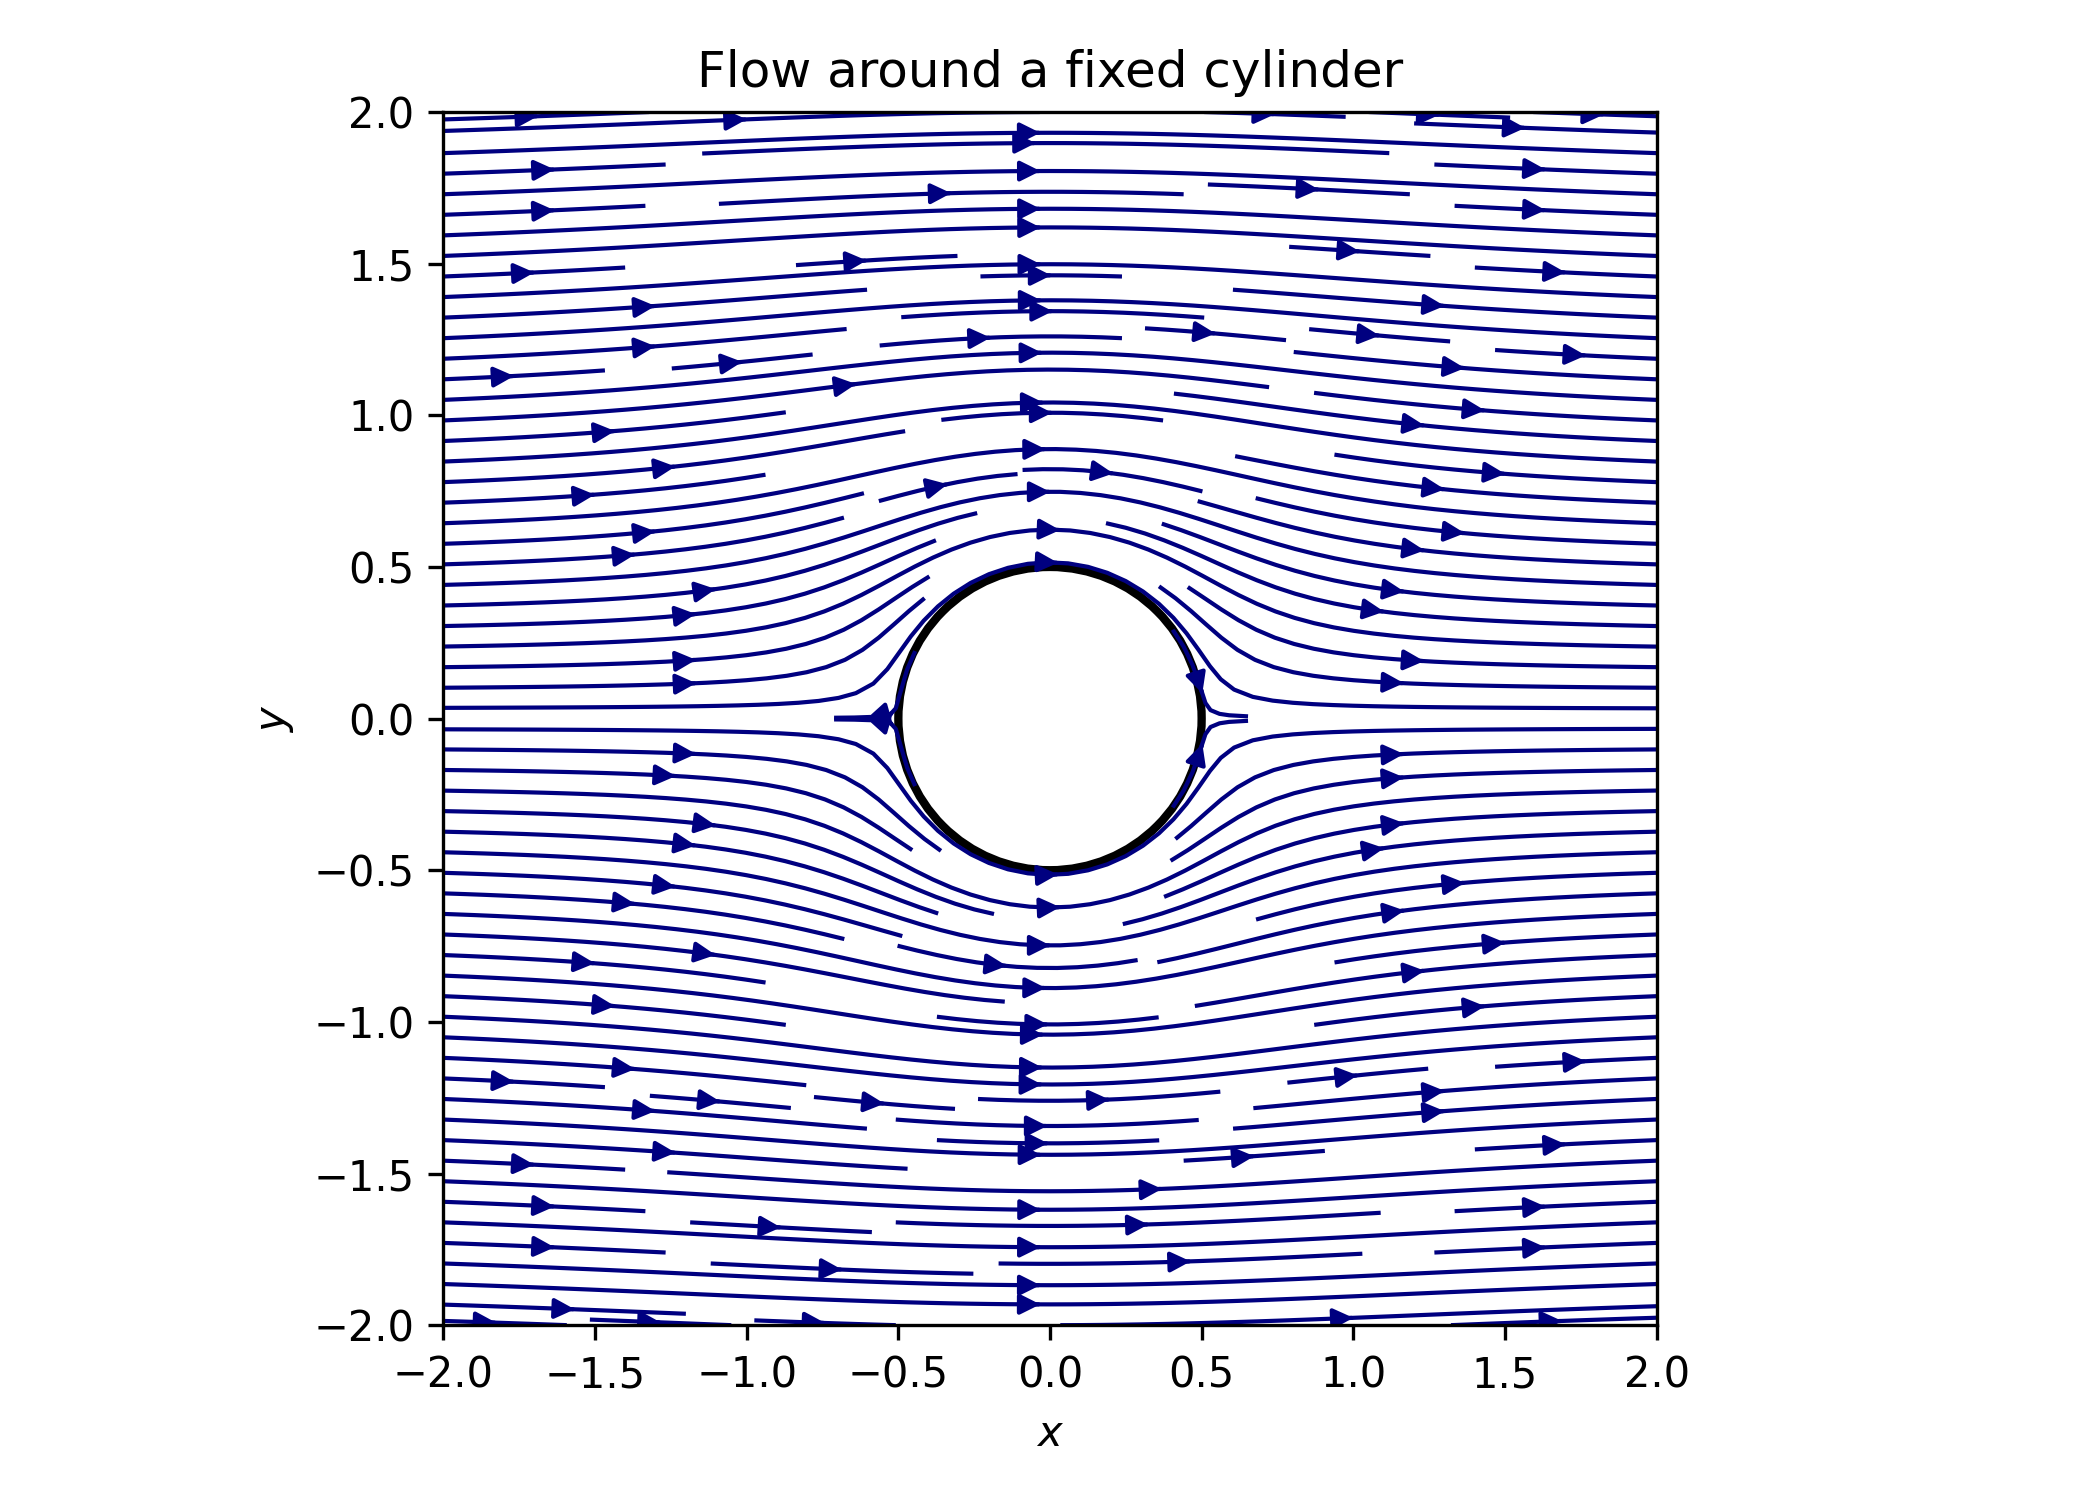
\includegraphics[width=0.85\textwidth]{02_cylinder_flow}
    \caption{Visualization of flow around a fixed cylinder as an analogy for æther flow around a stable vortex in the æther model. The uniform background flow is locally distorted by the presence of the vortex structure. This classical potential flow profile forms the basis for later interpretations of æther interactions in the model.}
    \label{fig:cylinderflow}
\end{figure}

\section{Introduction}
In a modern revival of Lord Kelvin's vortex-atom hypothesis of 1867~\cite{Kelvin1867-vortex}, we consider an absolute Euclidean space filled with a superfluid-like æther. This contemporary æther interpretation builds upon and extends historical frameworks such as the Lorentz–Poincaré æther theory, which introduced absolute frames and mechanical interpretations of relativistic phenomena. Unlike those early theories, however, the present model explicitly incorporates modern fluid dynamics, topological vortex theory, and quantum mechanical structure, distinguishing it in both conceptual rigor and empirical relevance. Thus, it maintains historical continuity while offering a modernized and experimentally verifiable framework.

In this model, elementary particles are represented as stable vortex knots or nodes embedded in the æther, and \emph{time} is defined by the intrinsic angular rotation of their vortex cores. The challenge is to derive \emph{time dilation} laws—analogous to those in special and general relativity (SR and GR)—using ætheric parameters such as constant density, circulation, and Planck-scale time, rather than invoking 4D spacetime curvature. We require that any such formulation reproduces known relativistic effects—for example, the slowing of clocks near massive bodies (gravitational redshift) or at high relative velocities (special-relativistic dilation)—despite operating in a flat, 3-dimensional absolute background. In other words, the \emph{eddy dynamics} of the æther—as illustrated in Figure~\ref{fig:cylinderflow}—must replicate the curvature-induced metric effects of general relativity with high fidelity.

Historically significant experiments such as Michelson–Morley (1887), Pound–Rebka (1959), and Gravity Probe A (1976) offer indirect yet consistent support for an æther-based interpretation of relativistic phenomena. The Michelson–Morley experiment placed stringent constraints on uniform æther drift, while the Pound–Rebka experiment confirmed the gravitational redshift predicted by Einstein. Gravity Probe A further verified gravitational time dilation with high precision. These observations can be interpreted naturally within the vortex æther framework presented here, providing empirical coherence across historical and modern domains.

This paper develops a mathematically rigorous model for time dilation based on vortex rotation dynamics in an approximately incompressible, inviscid superfluid-like æther, assuming incompressibility in the far field, with local compressibility admitted near core regions. We begin by formalizing the fundamental postulates of the æther model and defining how the rotation of a microscopic vortex constitutes a physical clock. We then derive two classes of time dilation laws: one for motion through the æther (analogous to SR), and one for vorticity-induced inflows around mass (analogous to GR). We demonstrate that these results quantitatively reproduce standard relativistic predictions—such as gravitational redshift and orbital clock effects—while replacing spacetime curvature with structured æther flows and vortex angular velocity fields as the origin of time dilation.
    \input{TimeDilation/2_superfluid_æther_framework}
    \section{Vortex Clocks and Proper Time}

\begin{figure}[H]
    \centering
    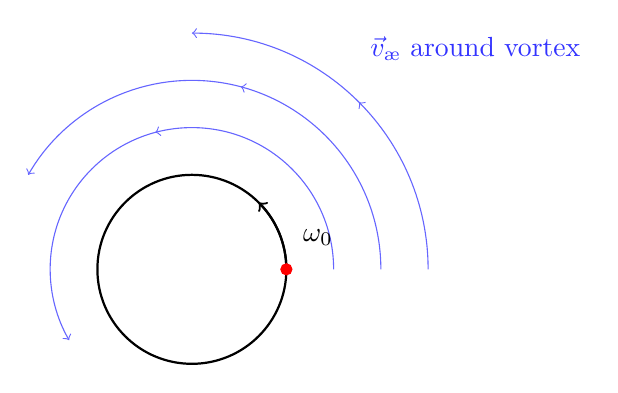
\begin{tikzpicture}[scale=2]
        \usetikzlibrary{decorations.markings}

        % Streamlines with varying arc lengths
        \draw[blue!60, ->,
            postaction={decorate},
            decoration={markings,
            mark=at position 0.5 with {\arrow{>}}}
        ] (0.9,0) arc (0:210:0.9); % Short arc

        \draw[blue!60, ->,
            postaction={decorate},
            decoration={markings,
            mark=at position 0.5 with {\arrow{>}}}
        ] (1.2,0) arc (0:150:1.2); % Medium arc

        \draw[blue!60, ->,
            postaction={decorate},
            decoration={markings,
            mark=at position 0.5 with {\arrow{>}}}
        ] (1.5,0) arc (0:90:1.5); % Long arc

        % Vortexring
        \draw[thick] (0,0) circle (0.6);
        \draw[thick, ->] (0:0.6) arc (0:45:0.6);
        \node at (0.8,0.2) {$\omega_0$};
        \filldraw[red] (0.6,0) circle (1pt);

        % Vectorveld label
        \node[blue!80] at (1.8,1.4) {$\vec{v}_{\ae}$ around vortex};

    \end{tikzpicture}
    \caption{Each $2\pi$ rotation of the vortex core = one tick of the internal clock.}
    \label{fig:wervelklok}
\end{figure}

In this model, a \grqq clock\textquotedblright is realized by a microscopic vortex's rotation. To make this concrete, consider a free particle at rest in the æther. Its vortex core spins steadily, dragging nearby æther around. Let $\omega_0$ denote the angular velocity of this core as measured in the æther rest frame (in units of radians per second). By definition, $\omega_0$ is the particle's \emph{proper rotational frequency}, corresponding to its proper time $\tau$.

We can relate $\omega_0$ to the passage of proper time: if the core rotates by $\Delta \theta$ radians in an interval, then the proper time elapsed is
\[
\Delta \tau = \frac{\Delta \theta}{\omega_0} \,.
\]
For example, if we choose $2\pi$ radians of rotation as a \("\)tick\("\) of the clock, then the proper period is $T_0 = 2\pi/\omega_0$. One might imagine $\omega_0$ is set by the particle's internal structure – e.g., a proton's vortex might rotate at some $10^{23}$ rad/s such that $T_0 \sim 10^{-23}$ s for one revolution (this is speculative, but notably, de Broglie in 1924 proposed that every particle of rest mass $m$ has an internal clock of frequency $mc^2/h$~\cite{deBroglie1924-frequency}, on the order of $10^{21}$ Hz for an electron; a vortex model could provide a physical origin for this \emph{Zitterbewegung} frequency as core rotation).

For now, $\omega_0$ is a free parameter representing the clock rate at rest. When the particle is not free or not at rest, its observed rotation rate can change. We define $\omega_{\textrm obs}$ as the angular velocity of the vortex core as observed by a static æther frame observer (i.e., one at rest with respect to the æther) under whatever circumstances (motion or gravity). The ratio $\omega_{\textrm obs}/\omega_0$ will then give the rate of the clock relative to proper time.

In fact, since $\Delta \tau = \Delta \theta / \omega_0$ always holds for the clock itself, and $\Delta t$ (coordinate time) corresponds to $\Delta \theta / \omega_{\textrm obs}$ (the angle rotated in lab frame time), we have:
\[
\frac{\Delta \tau}{\Delta t} = \frac{\Delta \theta / \omega_0}{\Delta \theta / \omega_{\textrm obs}} = \frac{\omega_{\textrm obs}}{\omega_0} \,. \tag{1}
\]

This important relation links the physical slowdown of the vortex's spin $\omega_{\textrm obs}$ to the time-dilation factor. If $\omega_{\textrm obs} < \omega_0$, the clock runs slow (since $\Delta \tau < \Delta t$).

Our task in the next sections is to determine $\omega_{\textrm obs}$ for two cases:
\begin{enumerate}
    \item When the vortex (particle) moves at velocity $v$ through the æther,
    \item When the vortex sits in a gravitational potential (æther flow) created by a massive body.
\end{enumerate}
We will find that $\omega_{\textrm obs}/\omega_0$ in these cases reproduces the familiar Lorentz and gravitational time dilation factors, respectively.

Before we proceed, we emphasize that \emph{proper time $\tau$ in this model is fundamentally just a count of the rotation of the vortex}. This provides an objective, mechanistic picture of time: for example, one could imagine a small flag or marker on the vortex core completing laps around the core—each lap is an unambiguous physical event corresponding to a fixed amount of proper time. Different physical clocks (atoms, molecules, etc.) would all eventually trace their time to such microscopic circulations in the universal æther.

For a discussion of how composite clocks consisting of multiple vortex nodes collectively experience time dilation, see Appendix~\ref{appendix:ClocksInVortexStructures}.

As long as the laws of physics are such that these circulations are stable and identical for identical particles, this provides a standard of time. We then show how motion through the æther and æther currents affect $\omega_{\textrm obs}$.
    
\section{Time Dilation from Relative Motion}

First, consider time dilation for a particle moving at high speed relative to the æther rest frame. Empirically, we know that a clock moving at velocity $v$ experiences time slower by the Lorentz factor $\gamma = 1/\sqrt{1 - v^2/c^2}$. In this model, we derive the same effect by analyzing the influence of absolute æther motion on vortex core rotation.

\subsection*{(a) Kinematic Derivation}

Let a vortex be at rest in its own frame $S'$ but moving at velocity $v$ relative to the æther rest frame $S$. In $S'$, the vortex rotates with angular frequency $\omega_0$, and defines proper time $\tau$. Due to Lorentz time dilation, an observer in $S$ sees the clock slow down:

\begin{figure}[htbp]
    \centering
    \includegraphics[width=0.85\textwidth]{06-TijddilatatieBeweging}
    \caption{Effect of æther flow on the internal rotation velocity of a vortex particle. At rest (left), the vortex retains its maximum angular velocity~$\omega_0$. When moving through the æther (right), the flow causes a reduced observed angular velocity to~$\omega_{\mathrm{obs}} < \omega_0$.}
    \label{fig:TijddilatatieBeweging}
\end{figure}

\[
\omega_\text{obs} = \omega_0 \sqrt{1 - \frac{v^2}{c^2}} \,.
\]
From the relation between proper and coordinate time,
\[
\frac{d\tau}{dt} = \frac{\omega_\text{obs}}{\omega_0} = \sqrt{1 - \frac{v^2}{c^2}} \,. \tag{2}
\]

This matches the standard SR time dilation formula. In our model, the physical mechanism is that æther motion across the vortex disrupts its swirl rate, slowing the apparent rotation in the æther frame.

\subsection*{(b) Fluid-Dynamic Interpretation}

A complementary interpretation uses compressible flow analogies. In fluid dynamics, a body moving at speed $v$ in a compressible medium with signal speed $c$ experiences distortions proportional to $\gamma = 1/\sqrt{1 - v^2/c^2}$. This can be thought of as a Doppler time dilation or resistance to maintaining coherent circulation. 

As velocity approaches the æther signal speed $c$, the surrounding flow compresses and resists vortex rotation. Therefore, the angular velocity seen in the æther frame drops, and:
\[
\omega_\text{obs} = \omega_0 \sqrt{1 - \frac{v^2}{c^2}} \Rightarrow \frac{d\tau}{dt} = \sqrt{1 - \frac{v^2}{c^2}} \,. \tag{3}
\]


In fluid dynamics, the Prandtl–Glauert factor explicitly characterizes compressible flow disturbances around objects moving near a medium\rqs s characteristic signal speed $c$. As velocity approaches this speed, fluid disturbances become increasingly resistant to propagation forward, closely analogous to the ætheric reduction of vortex core rotation at high velocities. Thus, the emergence of the Lorentz factor $\gamma$ in our model is physically and mathematically analogous to fluid compressibility effects.


\subsection*{Implication}

This gives us the relativistic time dilation for a moving clock:
\[
\boxed{\frac{d\tau}{dt} = \sqrt{1 - \frac{v^2}{c^2}}}
\]
within a Euclidean, æther-based flat space, and matches all special relativity experimental predictions~\cite{Rado2020-æther-Lorentz,Levy2009-æther-clock}.
    \section{Gravitational Time Dilation}

In General Relativity, clocks deeper in a gravitational potential well run slower compared to those at higher potentials. We reproduce this result using æther flow fields instead of spacetime curvature.

\subsection*{Æther Flow as Gravity}

We assume that mass $M$ induces an inward radial flow of æther. At a radius $r$, this flow speed is given by:
\[
v_g(r) = \sqrt{\frac{2GM}{r}}.
\]

\begin{figure}[htbp]
    \centering
    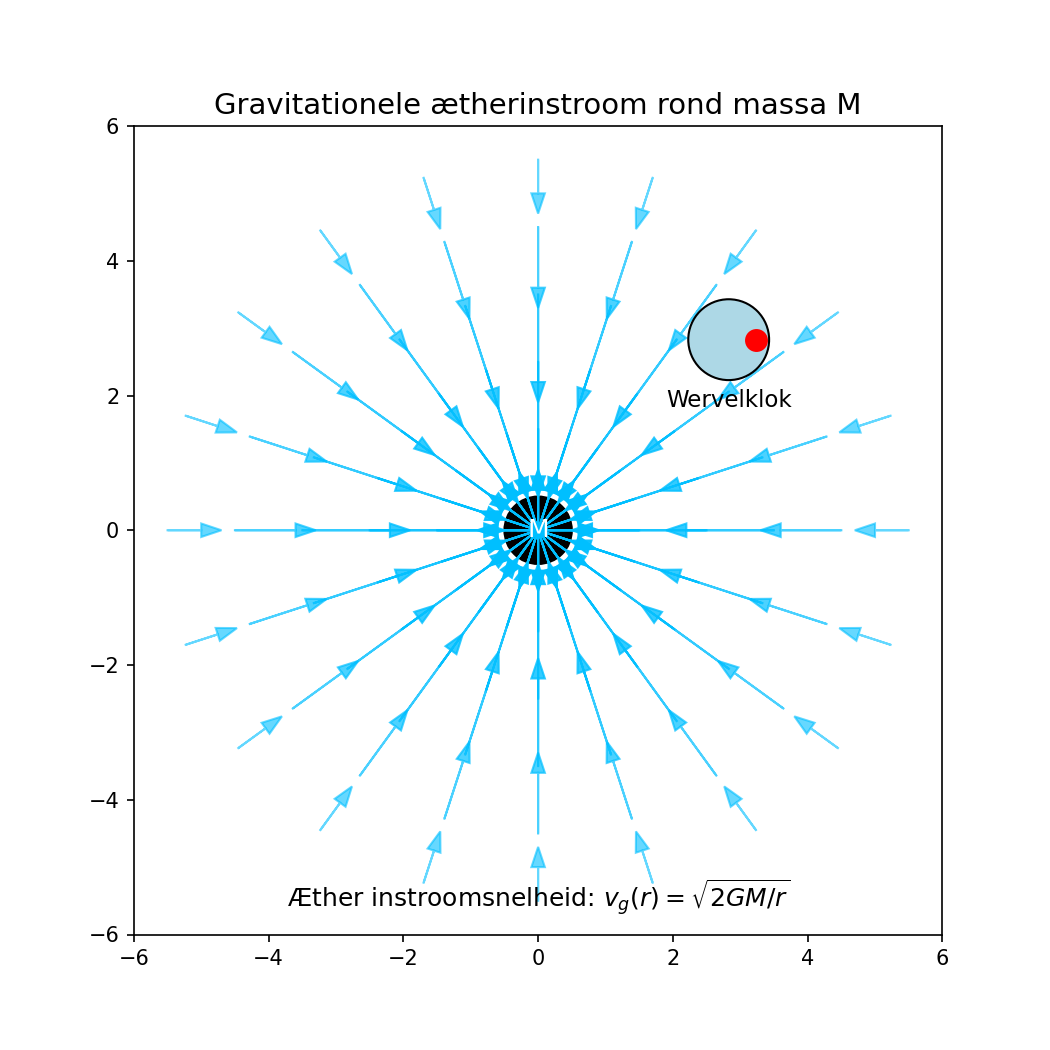
\includegraphics[width=0.85\textwidth]{images/07-GravitationeleÆtherinstroom}
    \caption{Gravitational time dilation due to radial æther inflow towards a mass~$M$. The vortex clock experiences a lower angular velocity due to æther drag, analogous to the Schwarzschild redshift.}
    \label{fig:GravitationeleÆtherinstroom}
\end{figure}

This mirrors the Painlevé–Gullstrand metric and the river model of black holes~\cite{Hamilton2004-river}.

\subsection*{Æther Drag and Clock Slowdown}

A clock held at radius $r$ in this inward æther flow sees æther moving past it at speed $v_g(r)$. The vortex core's observed angular velocity is therefore reduced due to the æther's drag, just as in the special relativity case, where motion through æther reduces the observed clock rate.

Thus, the gravitational time dilation factor is:
\[
\frac{d\tau}{dt} = \sqrt{1 - \frac{v_g^2(r)}{c^2}} = \sqrt{1 - \frac{2GM}{rc^2}}. \tag{4}
\]

A notable implication of gravitational æther inflow is related to the maximum force principle, defined as $F^{\text{max}}_{\text{gr}} = c^4 /4G$. Physically, this represents the upper limit on æther drag forces, where the inward æther flow near gravitational horizons reaches velocities close to ccc. At the Schwarzschild radius, the inflow speed of æther matches this limit, effectively freezing the rotation of any vortex-based clocks due to extreme drag, thus providing a tangible fluid-mechanical interpretation of gravitational horizons.

This is consistent with the Schwarzschild solution for stationary observers in general relativity.

A precise confirmation of gravitational time dilation under controlled conditions was provided by the Gravity Probe A mission~\cite{vessot_levine_1980}, which launched a hydrogen clock to an altitude of 10,000 km.

This delay was not only derived theoretically, but was confirmed experimentally by Pound and Rebka in 1959, who measured a gravitationally induced frequency shift between two points at different altitudes within the Earth's gravitational field using the Mössbauer effect~\cite{pound_rebka_1959}.

\subsection*{Interpretation}

This equation means that the deeper a vortex is located in the gravitational potential (the faster the local æther flow), the slower it rotates from the perspective of an observer at infinity. At the Schwarzschild radius $r_s = 2GM/c^2$, $d\tau/dt = 0$: time stops for external observers.

This provides a mechanistic interpretation of gravitational redshift: light emitted by a vortex-clock in a strong potential well appears redshifted due to the slower angular motion of the emitting vortex. The result:
\[
\boxed{\frac{d\tau}{dt} = \sqrt{1 - \frac{2GM}{rc^2}}}
\]
is fully consistent with GR and supports the æther flow analogy~\cite{Schiller2022-maxforce}.

\subsection*{Alternative Derivation via Æther Pressure Gradients}

An alternative and equally valid way to derive gravitational time dilation involves the use of Bernoulli's law for superfluids. Here, the gravitational potential is interpreted directly as a reduction in æther pressure near masses. According to Bernoulli's principle, a lower æther pressure corresponds to a higher local flow speed. Consequently, this pressure gradient interpretation aligns perfectly with the gravitational inflow velocity interpretation, providing theoretical versatility and enhancing the robustness of gravitational effects within the æther model.
    \section{Combined Effects and Further Predictions}

Having derived separate time dilation factors for motion through æther and gravitational æther flow, we now consider both effects simultaneously.

\subsection*{Combined Motion and Gravitational Field}

Let a vortex-clock move with velocity $\vec{u}$ in a region where the æther is flowing with velocity $\vec{v}_g$. The effective relative velocity with respect to the local æther flow is:
\[
\vec{v}_{\text{rel}} = \vec{u} - \vec{v}_g.
\]
The observed time dilation is then:
\[
\frac{d\tau}{dt} = \sqrt{1 - \frac{|\vec{v}_{\text{rel}}|^2}{c^2}}. \tag{5}
\]
This formulation smoothly incorporates both special and general relativistic effects into a single expression.

\subsection*{Example: Circular Orbit Time Dilation}

Consider a clock orbiting a mass $M$ at radius $r$. The tangential velocity of the orbit is:
\[
v_{\text{orb}} = \sqrt{\frac{GM}{r}}, \quad v_g(r) = \sqrt{\frac{2GM}{r}}.
\]
Since the orbital velocity is perpendicular to the radial æther inflow, the relative speed is:
\[
v_{\text{rel}} = \sqrt{v_{\text{orb}}^2 + v_g^2} = \sqrt{\frac{3GM}{r}}.
\]

\begin{figure}[htbp]
    \centering
    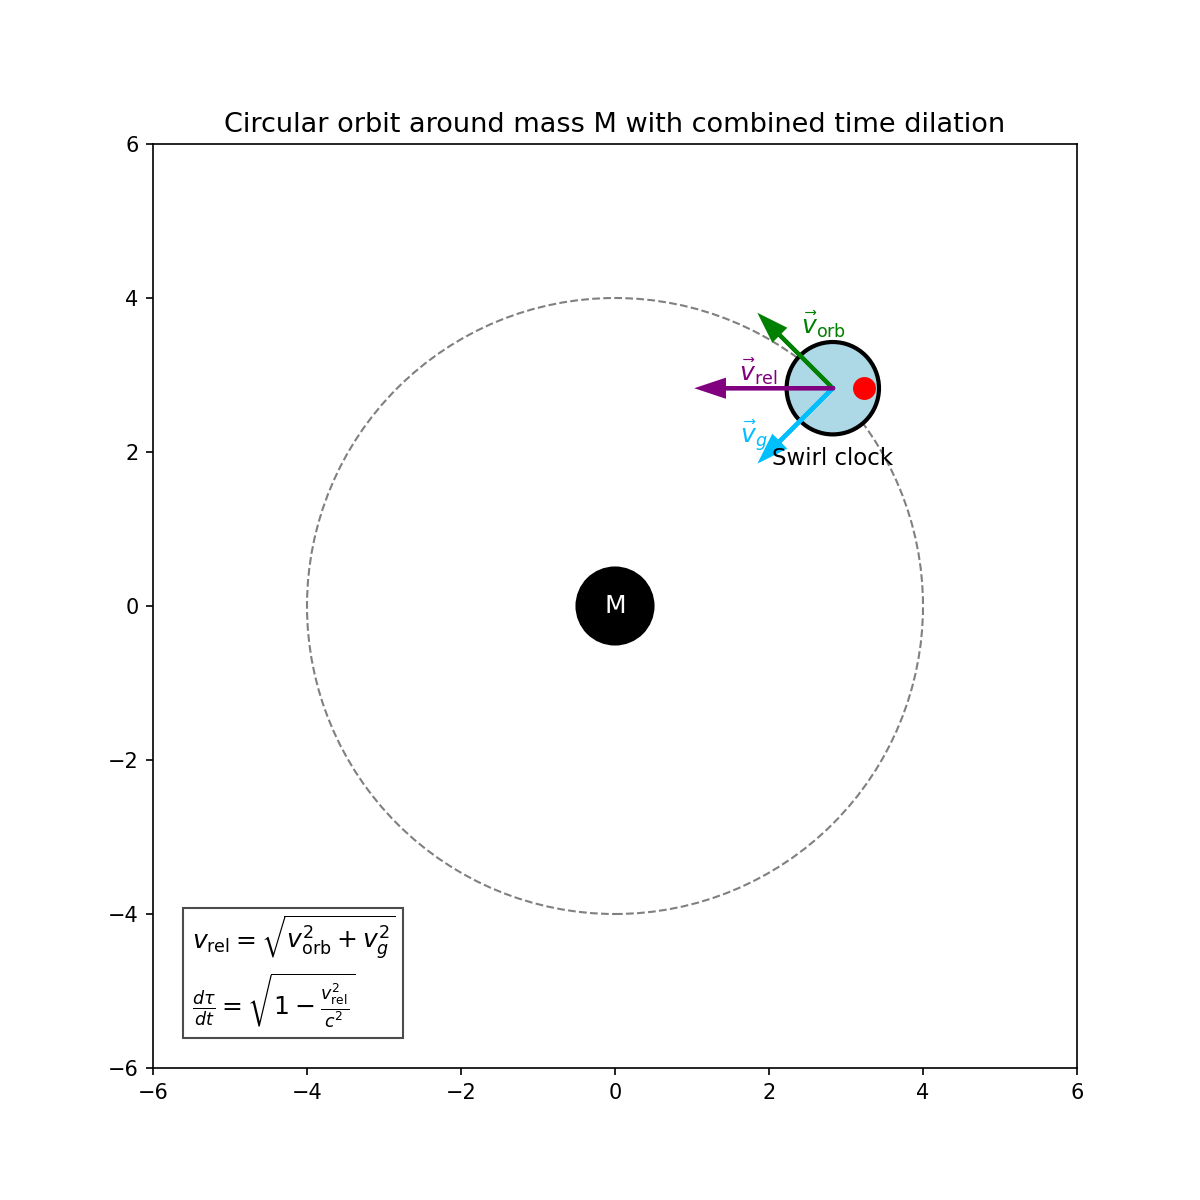
\includegraphics[width=0.85\textwidth]{../08-BaanRondMassa}
    \caption{A vortex in a circular orbit experiences combined time dilation due to orbital and æther flow. The clock experiences both orbital velocity~$\vec{v}_{\mathrm{orb}}$ and æther inflow~$\vec{v}_g$, which together result in a combined relative velocity~$\vec{v}_{\mathrm{rel}}$.}
    \label{fig:BaanRondMassa}
\end{figure}

Thus, the time dilation becomes:
\[
\frac{d\tau}{dt} = \sqrt{1 - \frac{3GM}{rc^2}}. \tag{6}
\]
This matches the exact result from Schwarzschild geometry for circular orbits.

\begin{figure}[htbp]
    \centering
    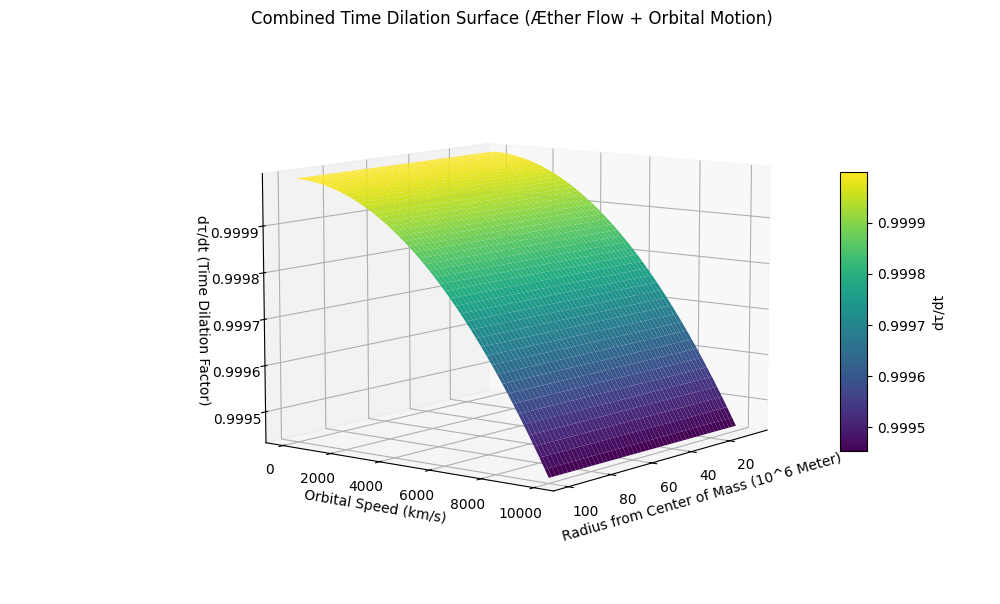
\includegraphics[width=0.85\textwidth]{../09-en-TimeDialationCombined}
    \caption{Visual representation of the time dilation factor \( \frac{d\tau}{dt} \) as a function of both the orbital velocity \( v_{\text{orb}} \) and the gravitational æther inflow velocity \( v_g \). The surface shows how both contributions — inertial and gravitationally derived æther flow — together result in a total slowing down of the clock. The hyperbolic curvature of the surface reflects the combined Lorentz and Schwarzschild dilation as described in equations (5) and (6).}
    \label{fig:TimeDialationCombined}
\end{figure}

\subsection*{Implications Near a Horizon}

As $r \to r_s = 2GM/c^2$, the inflow speed $v_g(r)$ approaches $c$, and any static observer's clock slows to zero. The æther flow fully suppresses local vortex rotation, providing a natural mechanism for the \("\)freezing of time\("\) at the event horizon.

\begin{figure}[htbp]
    \centering
    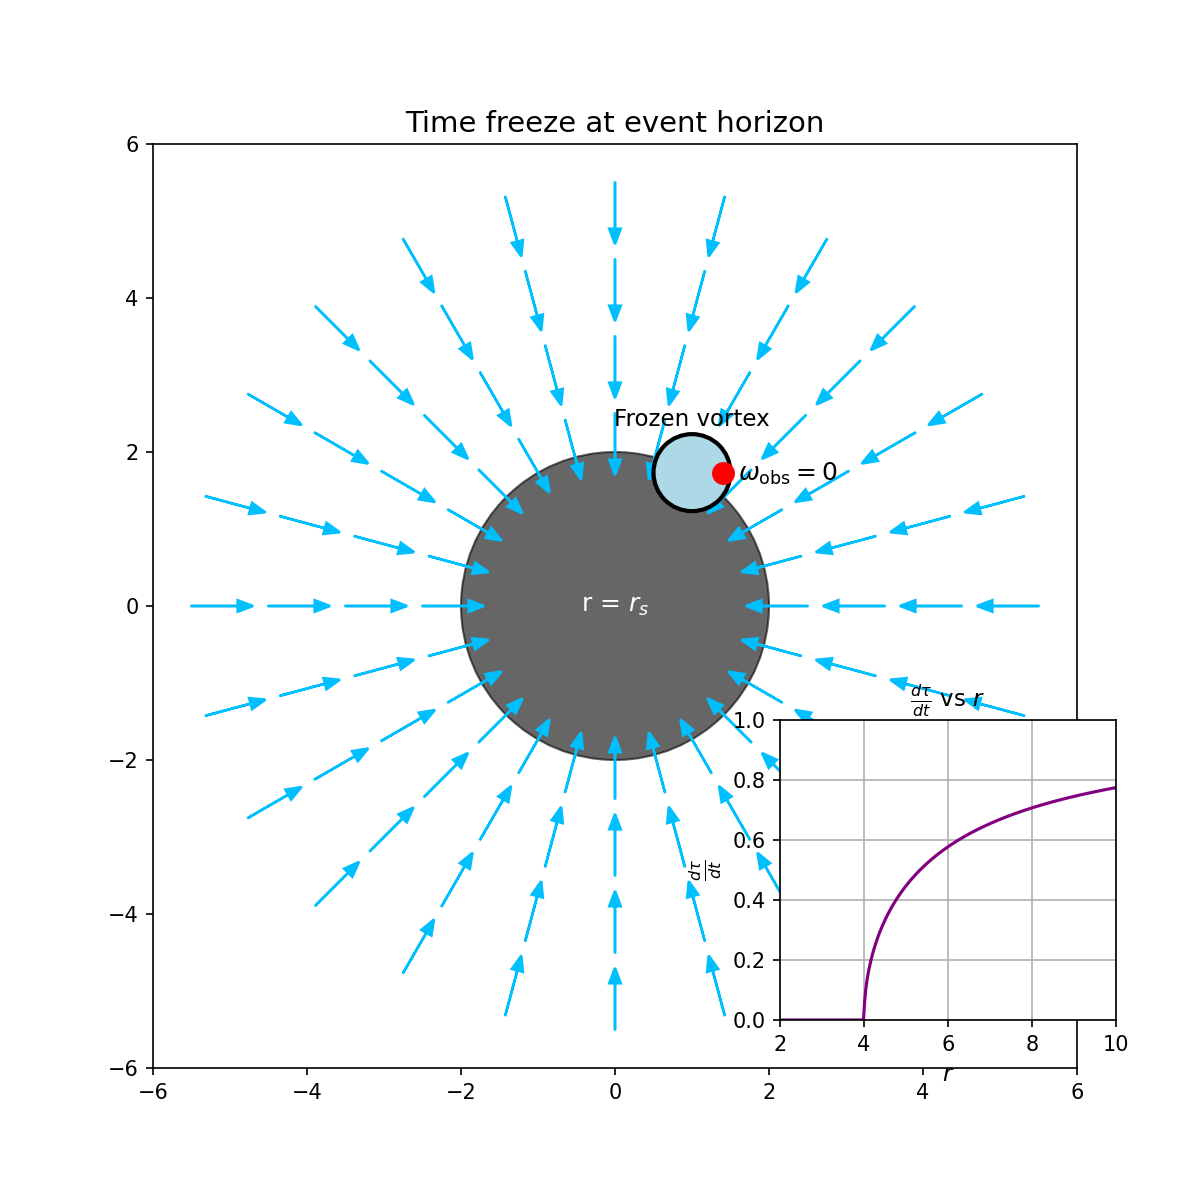
\includegraphics[width=0.85\textwidth]{../10-HorizonTijdsbevriezing}
    \caption{Æther flow accelerates towards $r_s$, where the observed clock rotation becomes zero. Freezing of time at the event horizon $r = r_s$: the Æther flow approaches~$c$, causing $\omega_{\mathrm{obs}} \to 0$. On the right, the corresponding decrease in $\frac{d\tau}{dt}$ as a function of distance is shown.}
    \label{fig:HorizonTijdsbevriezing}
\end{figure}


\subsection*{Quantum and Cosmic-Scale Consistency}

This vortex-æther framework naturally explains relativistic phenomena consistently across scales—from quantum to cosmic. For instance, at quantum scales, the observed lifetime dilation of rapidly moving muons directly results from reduced internal vortex rotation frequency in relativistic æther flows. At cosmic scales, near black hole horizons, vortex rotation essentially freezes due to æther inflow approaching ccc, providing a concrete physical mechanism for horizon phenomena. Such scale invariance underscores the comprehensive explanatory power of the æther model.

\subsection*{Unified Interpretation}

\begin{figure}[htbp]
    \centering
    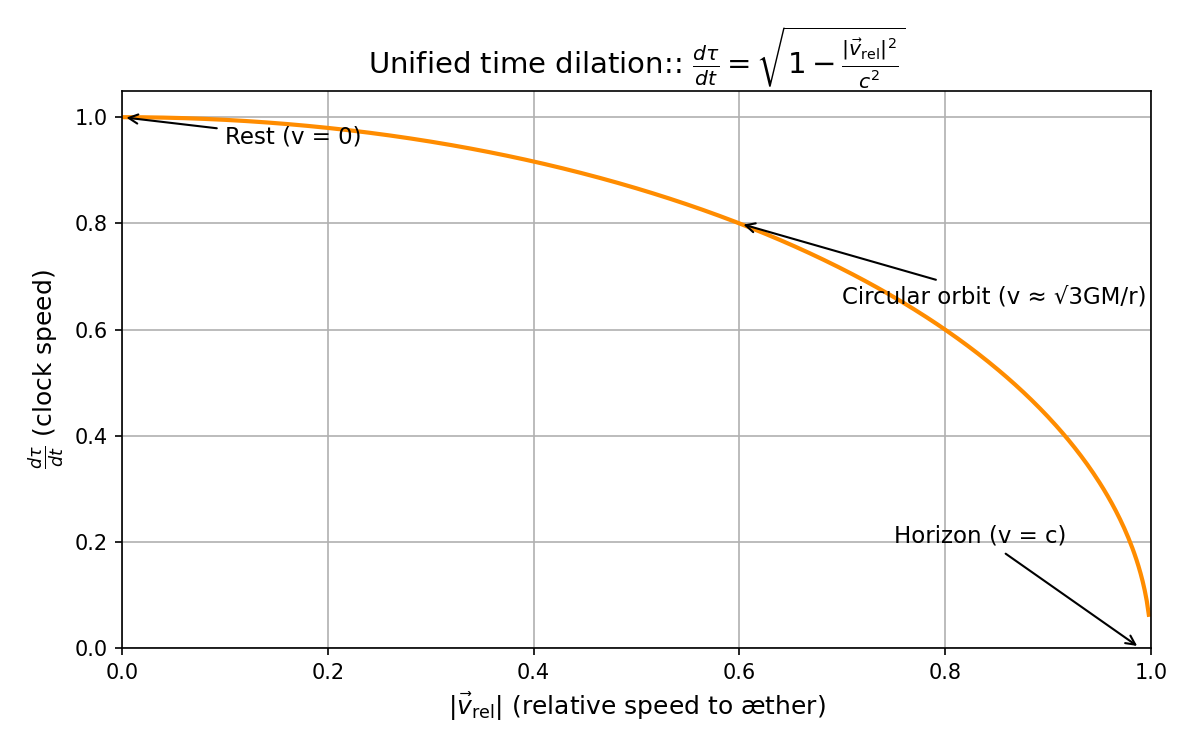
\includegraphics[width=0.85\textwidth]{../11-TijdsvertragingRelatieveBeweging}
    \caption{Universal time dilation formula in the Vortex Æther Model. The clock rate decreases with increasing relative velocity~$|\vec{v}_{\mathrm{rel}}|$ with respect to the æther. At $|\vec{v}_{\mathrm{rel}}| = c$ time stops.}
    \label{fig:TijdsvertragingRelatieveBeweging}
\end{figure}

This æther model allows all relativistic time dilation effects to be viewed as consequences of one principle:
\[
\text{Clock rate reduction} \;\propto\; \text{relative motion through æther}.
\]
Whether this relative motion arises from inertial velocity or from ætheric inflow due to nearby mass, the observable consequence is the same. Therefore, we conclude:
\[
\boxed{\frac{d\tau}{dt} = \sqrt{1 - \frac{|\vec{u} - \vec{v}_g|^2}{c^2}}}
\]
as the general time dilation formula for the Vortex Æther Model.
For possible experimental deviations of these time dilation formulas from general relativity, see Appendix-B~\ref{appendix:DeviatingPredictions}.
    
\section{Conclusion}

We have derived time dilation laws within a 3D Euclidean æther model, where particles are modeled as vortex knots, and time is defined by their intrinsic vortex core rotation. Motion through the æther and ætheric inflows (gravitational fields) reduce the observable angular velocity of vortex rotation, yielding:

\begin{itemize}
    \item The special-relativistic time dilation:
    \[
    \frac{d\tau}{dt} = \sqrt{1 - \frac{v^2}{c^2}},
    \]
    which arises from absolute motion through the æther.
    
    \item The gravitational time dilation:
    \[
    \frac{d\tau}{dt} = \sqrt{1 - \frac{2GM}{rc^2}},
    \]
    which arises from inward æther flow near mass $M$.
    
    \item The unified general case:
    \[
    \frac{d\tau}{dt} = \sqrt{1 - \frac{|\vec{u} - \vec{v}_g|^2}{c^2}},
    \]
    covering motion in a gravitational field.
\end{itemize}

These results accurately reproduce predictions of special and general relativity using physically intuitive mechanisms grounded in fluid dynamics.

The æther model eliminates the need for curved spacetime by replacing it with structured velocity fields in flat space. It reinterprets relativistic time effects as real, mechanical consequences of vortex core dynamics interacting with a physical æther.

This approach couples microphysics (vortex core rotation) with cosmological structure (black hole horizons) and maintains continuity across scales. By interpreting time dilation as angular deceleration of vortices, this model provides a mechanistic, field-based alternative to geometric spacetime curvature, preserving experimental consistency with SR and GR while opening possibilities for fluid dynamical extensions of fundamental physics~\cite{Winterberg2002-PlanckÆther,Schiller2022-maxforce}.

Future work may include deriving Einstein\rqs s field equations of conservation of æther vorticity or testing laboratory analogues via superfluid experiments. The reinterpretation of black hole horizons, gravitational redshift, and quantum timekeeping via vortex rotation encourages deeper theoretical and experimental investigations into the role of æther in modern physics.

A more extensive elaboration of these ideas can be found in the follow-up study: \textit{\grqq Swirl Clocks and Vorticity-Induced Gravity\textquotedblright } (2025).~\cite{vam2025unified}.

    \appendix \label{sec:Part-6}
    \section*{Appendix A: Macroscopic Clocks as Composite Vortex Structures}
\label{appendix:ClocksInVortexStructures}

In the Vortex Æther Model (VAM), time is defined as the internal rotation of a vortex core. This raises the question of how macroscopic clocks, such as atomic clocks or photonic oscillators, experience time dilation when they consist of an ensemble of vortices.

\subsection*{Time dilation of individual vortices}

According to the model, a single vortex node undergoes time dilation given by:
\begin{equation}
d\tau = \frac{1}{\Omega} \, d\theta = dt \cdot \sqrt{1 - \frac{v_{\text{rel}}^2}{c^2}} \label{eq:single_tau}
\end{equation}
where \( \Omega \) is the intrinsic angular velocity of the vortex core, and \( v_{\text{rel}} \) is the relative velocity of the vortex with respect to the local æther flow.

\subsection*{Compound vortex systems}

Consider a macroscopic system with \( N \) vortices, each with local angular velocity \( \Omega_i \). The effective time increase for the total system is:
\begin{equation}
\langle d\tau \rangle = \frac{1}{N} \sum_{i=1}^{N} \frac{1}{\Omega_i} \, d\theta_i \label{eq:ensemble}
\end{equation}

When the system is coherent — for example in a crystal or atomic clock — then \( \Omega_i \approx \Omega \), and thus:
\begin{equation}
\langle d\tau \rangle \approx \frac{1}{\Omega} \, d\theta \tag{\ref{eq:ensemble}'}
\end{equation}
which is equal to the time dilation of a single vortex (equation~\ref{eq:single_tau}).

\subsection*{Decoherent systems}

In decoherent or chaotic systems, the relative velocities \( v_{\text{rel}, i} \) vary per vortex. Then:
\begin{equation}
\langle d\tau \rangle = \left\langle \sqrt{1 - \frac{v_{\text{rel}, i}^2}{c^2}} \right\rangle dt
\end{equation}
Which is initially approximated as:
\begin{equation}
\langle d\tau \rangle \approx dt \cdot \sqrt{1 - \frac{\langle v_{\text{rel}}^2 \rangle}{c^2}} \label{eq:average_dil}
\end{equation}

\subsection*{Conclusion}

In both coherent and decoherent systems, the total time dilation is consistent with the individual dilation of the underlying vertebral nodes. This explains why complex systems — atomic clocks, crystals, biological rhythms — universally slow down in gravitational fields or at high velocities: their internal structure is built from the same rotating vorticity cores.

\vspace{1em}
\noindent
This derivation confirms that the VAM model is scale-independent and reproduces time dilation at both the micro- and macroscopic levels.
    \section*{Appendix B: Deviating Predictions from General Relativity}
\label{appendix:DeviatingPredictions}

The Vortex Æther Model (VAM) reproduces many well-known results of general relativity (GR), but also suggests a number of experimentally testable deviations in regimes where classical geometric theory does not provide an explicit explanation. Below we formulate three concrete situations in which the VAM model makes predictions that (in principle) deviate from GR.

\subsection*{1. Time dilation in rotating superfluids}

In rotating superfluids such as liquid helium or Bose-Einstein Condensates (BECs), macroscopic quantum vortices with measurable angular velocity \( \omega \) arise. Within VAM, local time dilation applies via:

\begin{equation}
d\tau = dt \cdot \sqrt{1 - \frac{\omega^2 R^2}{c^2}},
\end{equation}

where \( R \) is the distance to the vortex center. This effect is measurable via clock shifts on the µs scale if atomic clocks are placed at different locations within a rotating BEC.

\subsection*{2. Vorticity-dependent delay in LENR-like systems}

VAM predicts that in highly oscillatory electromagnetic cavitation (such as in low-energy nuclear reactions) a local swirl potential arises:

\begin{equation}
\Phi_\text{swirl} = \frac{1}{2} \omega^2 r^2 \Rightarrow \Delta \tau \sim \frac{\Phi_\text{swirl}}{c^2} \cdot dt.
\end{equation}

This would cause internal time in vortex-rich nanostructures to slow down measurably. Application to Pd/D electrodes with µs resolution could detect this delay via optical measurement intervals or anomalies in gamma noise profiles.

\subsection*{3. Light Bending Without Spacetime Curvature}

Instead of geodesic deflection in a curved space, VAM considers light as flowing in an æther with inhomogeneous velocity. The deflection then follows from a refraction gradient:

\begin{equation}
    \nabla n(\vec{r}) = \frac{1}{c} \frac{\partial v_\text{\ae}}{\partial r} \Rightarrow \delta \theta = \int \frac{dn}{dr} \, dr,
\end{equation}

which is experimentally testable via analogous gravity simulations in rotating fluid trays or optical metamaterials with swirl index gradient.

\bigskip

These scenarios show that the VAM model predicts experimentally distinctive behavior in situations where GR is neutral or unpredictable. Further experimental validation is necessary to establish the applicability of these predictions.
    \section*{Appendix C:}\label{appendix:temporal_structures}
\section*{Temporal Structures in the Vortex Æther Model (VAM)}

This appendix formalizes the temporal constructs introduced in the VAM framework. These layered notions of time enable nuanced distinctions between internal vortex dynamics, observable relativistic time, and the underlying absolute flow of the æther.

\subsection*{Aithēr-Time $\mathcal{N}$ — Absolute Background Time}
Concept: The universal, nonlocal flow of time; the foundation from which all other temporal phenomena are derived.


\[
\mathcal{N} \in \mathbb{R}, \quad d\mathcal{N} = \text{invariant}
\]

\textbf{Physical Role:} Provides the absolute time frame used to define causality and field evolution in the æther medium.

\subsection*{Now-Point $\nu_0$ — Local Present Intersection}
Concept: The intersection of a system with the absolute time—defining its local \("\)now.\("\)


\[
\nu_0(x) : \tau(x) = \mathcal{N}
\]

\textbf{Role:} Anchors relativistic causality. Each observer's \("\)present\("\) exists as a now-point in the universal flow.

\subsection*{Swirl Clock $S(t)$ — Phase Evolution, Continuous Identity}
Concept: The cyclic time evolution of a vortex; a phase tracker or heartbeat of the vortex.


\[
S(t) = \theta(t) \mod 2\pi
\]

\textbf{Role:} Represents the local angular phase of the vortex; tracks internal identity through cyclic motion.

\subsection*{Vortex Time $T_v$ — Topological Duration, Internal Clock}
Concept: The intrinsic looped time experienced by a vortex through one full geodesic cycle.


\[
T_v = \oint \frac{ds}{v_{\text{phase}}}
\]

\textbf{Role:} Measures internal duration of a knot loop; basis for vortex identity and mass stability.

\subsection*{Chronos-Time $\tau$ — Measurable, External Flow}
Concept: Classical proper time experienced by moving bodies, projected from the universal frame.


\[
d\tau = \frac{1}{\gamma(\vec{v})} d\mathcal{N}
\]

\textbf{Role:} Governs relativistic time dilation and clock rates in the moving æther frame.

\subsection*{Kairos Moment $\mathbb{K}$ — Transformational Threshold}
Concept: A phase-critical moment in which irreversible change or collapse occurs.


\[
\mathbb{K}(\vec{x}, \tau) = \delta(\tau - \tau_c)
\]

\textbf{Role:} A singular moment of transition—birth, collapse, phase shift, or knot reconnection.


    \bibliography{../references}
    \bibliographystyle{unsrt}
\end{document}